\documentclass[conference]{IEEEtran}

\usepackage{cite}
\usepackage[pdftex]{graphicx}
\usepackage{amsmath}
\usepackage{amssymb}
\usepackage{booktabs}
\usepackage{url}
\usepackage{xcolor}
\usepackage[caption=false,font=footnotesize]{subfig}
\usepackage{float}
\usepackage{tikz}
\usetikzlibrary{arrows.meta}

\graphicspath{{figures/}}

\hyphenation{Min-kow-ski point-cloud post-pro-cess-ing}

\begin{document}

\title{Rate-Conditioned Post-Processing for Learned Point Cloud Compression}

\author{
  \IEEEauthorblockN{Spyridon Siannas}
  \IEEEauthorblockA{Department of Electrical and\\Computer Engineering\\
  University of Patras\\
  Patras, Greece\\
  up1053718@ac.upatras.gr}
  \and
  \IEEEauthorblockN{Konstantinos Moustakas}
  \IEEEauthorblockA{Department of Electrical and\\Computer Engineering\\
  University of Patras\\
  Patras, Greece\\
  moustakas@ece.upatras.gr}
}

\maketitle

% =============================================================================
\begin{abstract}
Point cloud compression underpins emerging volumetric video and telepresence
applications, where geometric fidelity at low bitrates is critical.
At low bitrates, learned codecs lose fine surface detail: edges blur, ridges
flatten, and standard point-to-point metrics fail to capture the loss.
Restoring this detail requires inferring local geometric priors from decoded
point positions, without relying on explicit feature engineering.
We propose a rate-conditioned post-processing network that restores edge
geometry on decoded point clouds.
A single 2.5M-parameter model handles multiple bitrates via a
Feature-wise Linear Modulation (FiLM)-conditioned prediction head,
without retraining per bitrate.
Because oversmoothing is spatially structured, with high-curvature regions
suffering most, the corrector must infer local surface geometry to determine
where and how strongly to intervene.
On the 8i Voxelized Full Bodies dataset, the method yields \textbf{+2.06~dB}
edge-region gain at low bitrate (r2), \textbf{+0.58~dB} at medium bitrate
(r4), and \textbf{+0.27~dB} at high bitrate (r6) over PCGCv2.
To make these gains legible, we introduce a curvature-stratified PSNR metric
that separately evaluates edge and flat surface regions, exposing degradation
that aggregate metrics mask.
Zero-shot transfer to a structurally different codec (Unicorn) and an unseen
dataset (MVUB) suggests low-rate oversmoothing is a failure mode common to
multiple learned codecs, and our approach successfully recovers fine surface
structure across codecs and datasets without retraining.
\end{abstract}

% =============================================================================
\section{Introduction}
\label{sec:intro}

Point cloud compression has attracted growing research interest with the spread
of LiDAR sensors, volumetric video capture, and mixed-reality
telepresence~\cite{schwarz2018emerging}. Learned codecs such
as PCGCv2~\cite{wang2021multiscale} and Unicorn~\cite{wang2025unicorn} achieve competitive rate-distortion performance against traditional
standards such as G-PCC~\cite{graziosi2020gpcc}, yet their behavior at low
bitrates reveals a consistent failure mode: oversmoothing of geometric detail~\cite{he2022density}.
The mechanism is well understood at the level of entropy-coded occupancy grids:
the entropy model assigns higher coding cost to rare fine-scale occupancy
patterns, which is precisely what high-curvature surface detail produces.
Unlike additive noise, oversmoothing is hard to reverse: once nearby surface
points collapse into a single decoded voxel, the original configuration is
unrecoverable from the decoded signal alone.

The pattern of such errors is not random. Decoded point clouds retain
coarse surface geometry faithfully; fine structure (ridges, creases, sharp
transitions) suffers most -- a systematic spatial bias that standard
aggregate metrics such as D1 PSNR (point-to-point) fail to expose,
as they average error uniformly over the surface without regard to local
surface geometry.
The degradation is also \emph{rate-dependent}: edge gains diminish
significantly as bitrate increases, confirming that at high bitrates the
codec already preserves fine structure well while at low bitrates corrections
must be stronger. A fixed model trained at a single operating point cannot
adapt to this range.

We address this with a sparse U-Net post-processor conditioned on the compressed
bitrate via Feature-wise Linear Modulation (FiLM)~\cite{perez2018film}. A
single model trained jointly across multiple bitrates shares geometric
representations while applying rate-specific corrections. Augmenting the input with explicit curvature features does not help: the
backbone's receptive field already captures local surface geometry from point
positions, and curvature adds noise at the high-curvature boundaries where
corrections matter most.

Our main contributions are:
\begin{itemize}
  \item A rate-conditioned post-processing network for learned point cloud
    codecs, using a FiLM-modulated sparse U-Net head with coordinate-only
    input features and Chamfer Distance loss.
  \item A curvature-stratified PSNR metric that separately quantifies quality
    at edge and flat surface regions, exposing systematic per-region degradation
    that aggregate metrics do not capture.
  \item Experimental evidence that coordinate-only features outperform
    curvature-augmented features, and that the method generalizes zero-shot
    to an unseen codec (Unicorn) and an unseen dataset (MVUB).
\end{itemize}

% --- Figure 1: Architecture ---
\begin{figure*}[t]
  \centering
  \resizebox{0.96\textwidth}{!}{%
  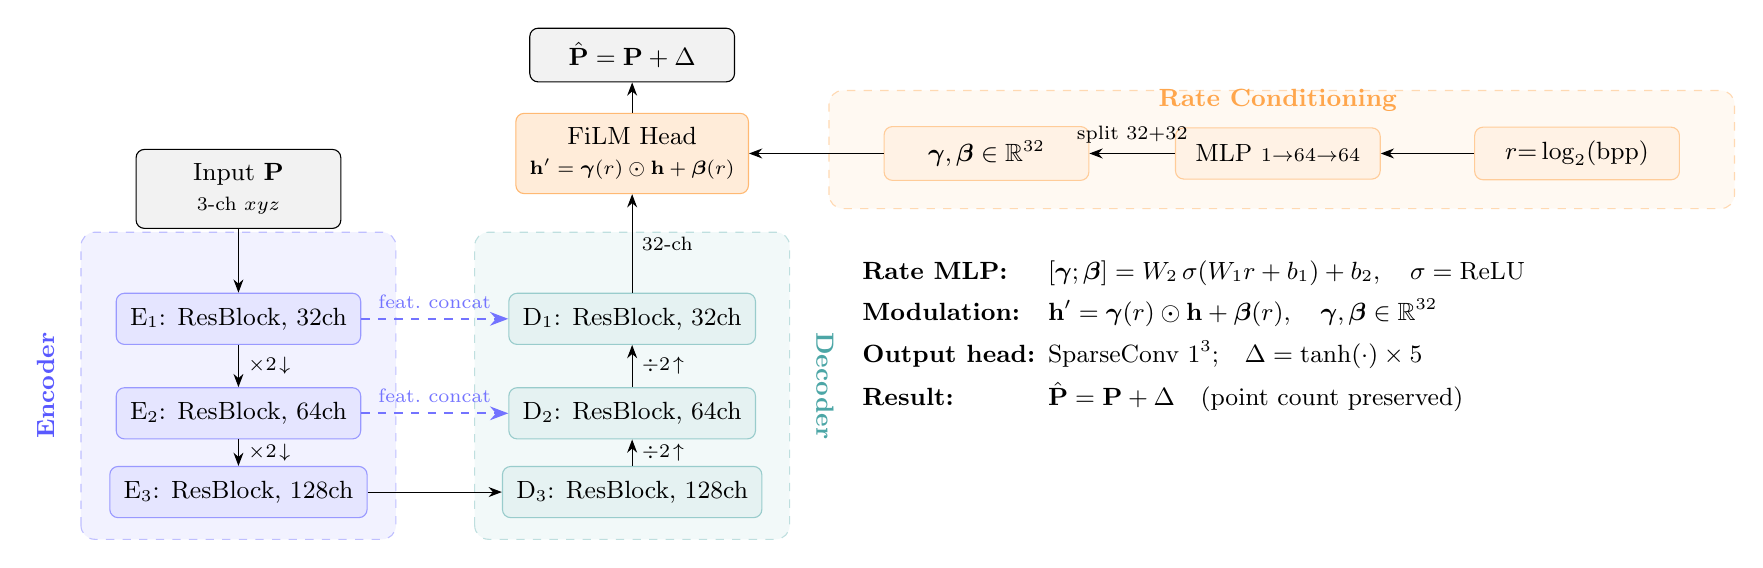
\begin{tikzpicture}[
    >=Stealth,
    every node/.style={font=\small},
    box/.style={draw, rounded corners=3pt, inner sep=5pt,
                align=center, minimum width=2.6cm, minimum height=0.65cm},
    enc/.style={box, fill=blue!10, draw=blue!40},
    dec/.style={box, fill=teal!10, draw=teal!40},
    film/.style={box, fill=orange!15, draw=orange!55},
    rate/.style={box, fill=orange!10, draw=orange!40},
    sec/.style={font=\small\bfseries},
  ]
  %% ---- Region boxes ----
  % Encoder (blue, left column)
  \draw[rounded corners=5pt, fill=blue!5, draw=blue!25, dashed]
    (-2.0,-3.6) rectangle (2.0, 0.3);
  % Decoder (teal, right column)
  \draw[rounded corners=5pt, fill=teal!5, draw=teal!25, dashed]
    (3.0,-3.6) rectangle (7.0, 0.3);
  % Rate Conditioning (orange, small box top-right)
  \draw[rounded corners=5pt, fill=orange!5, draw=orange!30, dashed]
    (7.5, 0.6) rectangle (19.0, 2.1);
  %% ---- Region labels ----
  \node[sec, blue!65,  rotate=90]  at (-2.45, -1.65) {Encoder};
  \node[sec, teal!70,  rotate=-90] at (7.45,  -1.65) {Decoder};
  \node[sec, orange!70] at (13.2, 1.97) {Rate Conditioning};
  %% ---- Nodes ----
  % Input (above encoder box)
  \node[box, fill=gray!10] (P)   at (0,   0.85) {Input $\mathbf{P}$\\{\scriptsize 3-ch $xyz$}};
  % Encoder
  \node[enc] (e1) at (0,   -0.8) {E$_1$: ResBlock, 32ch};
  \node[enc] (e2) at (0,   -2.0) {E$_2$: ResBlock, 64ch};
  \node[enc] (e3) at (0,   -3.0) {E$_3$: ResBlock, 128ch};
  % Decoder
  \node[dec] (d3) at (5.0, -3.0) {D$_3$: ResBlock, 128ch};
  \node[dec] (d2) at (5.0, -2.0) {D$_2$: ResBlock, 64ch};
  \node[dec] (d1) at (5.0, -0.8) {D$_1$: ResBlock, 32ch};
  % FiLM Head (above decoder, no separate box — identified by color)
  \node[film] (fh) at (5.0, 1.3)
    {FiLM Head\\{\scriptsize $\mathbf{h}' = \boldsymbol{\gamma}(r)\odot\mathbf{h}+\boldsymbol{\beta}(r)$}};
  % Output (above FiLM Head)
  \node[box, fill=gray!10] (out) at (5.0, 2.55) {$\hat{\mathbf{P}} = \mathbf{P} + \Delta$};
  % Rate Conditioning (horizontal, same y as fh → straight arrows)
  \node[rate] (gb)  at (9.5,  1.3) {$\boldsymbol{\gamma},\boldsymbol{\beta}\in\mathbb{R}^{32}$};
  \node[rate] (mlp) at (13.2, 1.3) {MLP\ {\scriptsize $1{\to}64{\to}64$}};
  \node[rate] (bpp) at (17.0, 1.3) {$r{=}\log_2(\mathrm{bpp})$};
  %% ---- Info text (empty space: right of enc/dec, below rate cond) ----
  \node[anchor=north west, font=\small] at (7.8, 0.1) {%
    \begin{tabular}{@{}l@{\enspace}l@{}}
      \textbf{Rate MLP:}    & $[\boldsymbol{\gamma};\boldsymbol{\beta}] =
                               W_2\,\sigma(W_1 r + b_1) + b_2,\quad \sigma=\mathrm{ReLU}$ \\[4pt]
      \textbf{Modulation:}  & $\mathbf{h}' = \boldsymbol{\gamma}(r)\odot\mathbf{h}+\boldsymbol{\beta}(r),
                               \quad \boldsymbol{\gamma},\boldsymbol{\beta}\in\mathbb{R}^{32}$ \\[4pt]
      \textbf{Output head:} & SparseConv $1^3$;\quad $\Delta = \tanh(\cdot)\times 5$ \\[4pt]
      \textbf{Result:}      & $\hat{\mathbf{P}} = \mathbf{P} + \Delta$\quad (point count preserved)
    \end{tabular}%
  };
  %% ---- Arrows ----
  \draw[->] (P)  -- (e1);
  \draw[->] (e1) -- node[right]{\scriptsize $\times2\!\downarrow$} (e2);
  \draw[->] (e2) -- node[right]{\scriptsize $\times2\!\downarrow$} (e3);
  \draw[->] (e3) -- (d3);
  \draw[->] (d3) -- node[right]{\scriptsize $\div2\!\uparrow$} (d2);
  \draw[->] (d2) -- node[right]{\scriptsize $\div2\!\uparrow$} (d1);
  \draw[->] (d1) -- node[right]{\scriptsize 32-ch} (fh);
  \draw[->] (fh) -- (out);
  \draw[->, dashed, blue!55, thick] (e1.east) -- node[above]{\scriptsize feat.\ concat} (d1.west);
  \draw[->, dashed, blue!55, thick] (e2.east) -- node[above]{\scriptsize feat.\ concat} (d2.west);
  \draw[->] (bpp) -- (mlp);
  \draw[->] (mlp) -- node[above]{\scriptsize split 32+32} (gb);
  \draw[->] (gb.west) -- (fh.east);
  \end{tikzpicture}%
  }
  \caption{Architecture overview. The rate-invariant sparse U-Net backbone
  (Encoder + Decoder) processes the decoded point cloud. Skip connections
  (dashed) concatenate encoder features to decoder inputs at matching
  resolutions. The FiLM head applies per-channel affine modulation
  $\mathbf{h}' = \boldsymbol{\gamma}(r)\odot\mathbf{h}+\boldsymbol{\beta}(r)$
  to the 32-channel pre-head features; modulated features then pass through a
  $1^3$ sparse convolution and $\tanh(\cdot)\times 5$ to produce displacement
  vectors $\Delta$. $\boldsymbol{\gamma},\boldsymbol{\beta}\in\mathbb{R}^{32}$
  are the split output of a small MLP from the log-BPP scalar $r$.}
  \label{fig:arch}
\end{figure*}

% =============================================================================
\section{Related Work}
\label{sec:related}

\subsection{Learned Point Cloud Compression}

Point cloud compression has traditionally been addressed by geometry-based
standards such as G-PCC~\cite{graziosi2020gpcc}. Learned codecs represent
3D point clouds mainly as occupancy grids processed by sparse convolutional
autoencoders. PCGCv2~\cite{wang2021multiscale,wang2023sparsepcgc}
introduced a multi-scale architecture operating on voxelized geometry;
subsequent work~\cite{wang2025unicorn} extended this to joint geometry-attribute
coding at variable rates. These codecs share the oversmoothing behavior
documented here, as both employ entropy-coded latent representations that
discard fine-scale detail at low bitrates~\cite{he2022density,wang2025unicorn}.

\subsection{Post-Processing for Point Cloud Compression}

Fan et al.~\cite{fan2022deep} proposed a graph network for post-processing
G-PCC decoded geometry, demonstrating BD-PSNR improvements; Pang et
al.~\cite{pang2022graspnet} followed with GRASP-Net, a residual analysis
and synthesis approach for G-PCC geometry. Artifact removal for image
compression has a longer history~\cite{dong2015compression}, motivating
analogous approaches for 3D geometry. Concurrent work on attribute
enhancement~\cite{ugae2025} targets color restoration after geometry
refinement. Within learned codec pipelines, Guarda et al.~\cite{guarda2025deep} and
Xu et al.~\cite{xu2024fast} integrate post-decoding refinement modules for
geometry recovery; these are codec-specific components rather than standalone
post-processors. To the best of our knowledge, no prior work applies external, rate-conditioned
post-processing to general learned point cloud codec output.

\subsection{Feature-wise Linear Modulation}

FiLM conditioning~\cite{perez2018film} was originally proposed for visual
question answering. Related approaches use similar affine feature modulation
for variable-rate image and video
compression~\cite{choi2019variable,cui2021asymmetric,song2021variable,li2024neural},
establishing it as an effective mechanism for single-model rate control.

% --- Figure 2: Qualitative visualization ---
\begin{figure*}[t]
  \centering
  \includegraphics[width=\textwidth]{figures/soldier_vis.png}
  \caption{Soldier sequence, frame 803, at r2 (0.05~bpp).
  \textbf{Left}: original (79,529 pts).
  \textbf{Centre}: PCGCv2 compressed (76,058 pts); surface protrusions and
  structural boundaries merge into the surrounding geometry.
  \textbf{Right}: proposed method (76,058 pts); fine geometric structure
  substantially recovered without changing overall shape.
  Point count is preserved by construction ($|\hat{\mathbf{P}}|=|\mathbf{P}|$).}
  \label{fig:vis}
\end{figure*}

% =============================================================================
\section{Method}
\label{sec:method}

\subsection{Problem Formulation}

Let $\mathbf{P} \in \mathbb{Z}^{N \times 3}$ denote a decoded point cloud on
an integer voxel grid, and let $\mathbf{P}^* \in \mathbb{Z}^{M \times 3}$
denote the original uncompressed cloud.

We seek a function $f_\theta(\mathbf{P}, r) \approx \mathbf{P}^*$
parameterized by $\theta$, where $r = \log_2(\mathrm{bpp})$ is a per-frame
scalar computed from the actual decoded bits of that specific frame.
Using the per-frame value rather than a nominal rate point allows the model
to generalize to codecs with variable-bpp output.

The output is a refined cloud $\hat{\mathbf{P}} = \mathbf{P} + \Delta$,
where $\Delta \in \mathbb{R}^{N \times 3}$ are predicted displacement vectors.
Point count is preserved by construction: $|\hat{\mathbf{P}}| = |\mathbf{P}|$.

\subsection{Network Architecture}
\label{subsec:arch}

The architecture is shown in Fig.~\ref{fig:arch}. The backbone is a
three-level sparse U-Net with residual blocks at each resolution, implemented
in Minkowski Engine~\cite{choy20194d}. Each encoder
block applies two sparse $3{\times}3{\times}3$ convolutions with instance
normalization and ReLU, followed by strided convolution for downsampling.
Skip connections concatenate encoder and decoder feature maps at matching
resolutions. The backbone operates without rate information, producing
rate-invariant geometric features.

The prediction head takes the 32-channel pre-output feature map $\mathbf{h}$
and applies a FiLM layer conditioned on the bitrate scalar $r$.
A shared MLP maps $r$ to 64 values split into per-channel
\textbf{scale} parameters $\boldsymbol{\gamma}$ and
\textbf{shift} parameters $\boldsymbol{\beta}$:
\begin{equation}
  [\boldsymbol{\gamma};\boldsymbol{\beta}] = W_2\,\sigma(W_1 r + b_1) + b_2,
  \quad W_1\!\in\!\mathbb{R}^{64\times1},\; W_2\!\in\!\mathbb{R}^{64\times64},
  \label{eq:mlp}
\end{equation}
where $\sigma$ is ReLU. The FiLM modulation is then
\begin{equation}
  \mathbf{h}' = \boldsymbol{\gamma}(r) \odot \mathbf{h} + \boldsymbol{\beta}(r),
  \label{eq:film}
\end{equation}
with $\boldsymbol{\gamma},\boldsymbol{\beta}\in\mathbb{R}^{32}$ and $\odot$
denoting channel-wise multiplication.
The modulated features pass through a $1{\times}1{\times}1$ convolution
followed by $\tanh(\cdot) \times d_{\max}$, where $d_{\max}=5$ voxels.
Confining all rate-dependent computation to the head prevents gradient
interference between rates in the shared backbone.

\subsection{Input Features}

Each decoded point is represented by its normalized $(x, y, z)$ coordinates
(3 channels). We do not include per-point curvature as an input feature.
Although curvature is useful for \emph{evaluating} geometric quality,
providing it as input slightly degrades post-processing performance
(Section~\ref{subsec:ablation}): the backbone encodes local geometry
from voxel coordinates directly.

\subsection{Training}
\label{subsec:training}

We train on multi-frame decoded sequences from PCGCv2 at three bitrate levels
(r2, r4, r6). Training patches of $64^3$ voxels are extracted with stride 32,
retaining only patches with at least 100 points (to exclude near-empty border
patches that carry no geometric signal). Augmentation applies random
axis permutation and sign flips (48 discrete orientations).

The loss is the symmetric Chamfer Distance~\cite{fan2017pointset} between the refined patch
$\hat{\mathbf{P}}$ and a crop of the original cloud $\mathbf{P}^*$:
\begin{equation}
  \mathcal{L}_{\mathrm{CD}} = \frac{1}{|\hat{\mathbf{P}}|}\sum_{\hat{p} \in
  \hat{\mathbf{P}}} \min_{p^* \in \mathbf{P}^*} \|\hat{p} - p^*\|_2
  + \frac{1}{|\mathbf{P}^*|}\sum_{p^* \in \mathbf{P}^*}
  \min_{\hat{p} \in \hat{\mathbf{P}}} \|p^* - \hat{p}\|_2
  \label{eq:cd}
\end{equation}
Original cloud crops are extracted with zero boundary padding to avoid
boundary-dominated gradients. Batches mix rates with weights $[1.0, 0.3, 0.05]$
for r2/r4/r6, reflecting the declining displacement signal: at r2 roughly
40\% of ground-truth displacements are non-zero, falling to below 15\% at r6;
uniform weighting would allow the easy, nearly-zero r6 patches to dominate.
This static choice was preferred over dynamic alternatives (Kendall
uncertainty weighting, gradient-normalized balancing), which consistently
degraded performance: the shared backbone prevents the learning-speed
decoupling these methods assume.
This is a deliberate bias toward low-rate correction and limits r4/r6
performance on out-of-distribution data, as discussed in
Section~\ref{subsec:generalization}.
We use AdamW with $\eta{=}5{\times}10^{-4}$, weight decay $10^{-4}$,
3-epoch linear warmup, and cosine annealing over 30 epochs on a single
NVIDIA RTX 3090 with batch size 16.

% =============================================================================
\section{Curvature-Stratified Evaluation}
\label{sec:metric}

Point cloud geometry quality is standardly measured by D1 PSNR
(point-to-point nearest-neighbor error) and D2 PSNR
(point-to-plane)~\cite{graziosi2020gpcc}, both aggregating error uniformly
over the cloud surface. This is appropriate for codec benchmarking but
counterproductive for post-processing evaluation: a corrector that recovers
edge geometry and one that improves flat regions instead can yield identical
aggregate scores, yet they are qualitatively different outcomes. Subjective
quality studies confirm that aggregate metrics fail to predict perceived
quality for learned-codec output~\cite{ak2024basics,prazeres2024quality},
where artifacts concentrate at geometrically complex regions rather than
distributing uniformly.

We propose a curvature-stratified PSNR. For each original point $p^*$,
surface curvature is estimated from the $k{=}30$ nearest neighbors
$\mathcal{N}_k(p^*)$ via PCA of the local covariance matrix:
\begin{equation}
  \kappa(p^*) = \frac{\lambda_0}{\lambda_0 + \lambda_1 + \lambda_2},
  \label{eq:curv}
\end{equation}
where $\lambda_0 \leq \lambda_1 \leq \lambda_2$ are the eigenvalues of
$\mathrm{Cov}(\mathcal{N}_k(p^*))$ (range $[0,\tfrac{1}{3}]$; higher values
indicate sharper surface curvature). Points are grouped into three equal-size
terciles by $\kappa$ over the original cloud. For each tercile stratum
$S \subset \mathbf{P}^*$, a one-sided PSNR is computed as
\begin{align}
  \mathrm{PSNR}_s &= 10\log_{10}\!\left(\frac{D_{\max}^2}{\mathrm{MSE}_s}\right),
  \notag \\
  \mathrm{MSE}_s &= \frac{1}{|S|}\sum_{p^*\in S}
  \min_{\hat{p}\in\hat{\mathbf{P}}} \|p^* - \hat{p}\|_2^2,
  \label{eq:stratpsnr}
\end{align}
where $D_{\max}=1023$ for 10-bit voxel grids. We call the top-tercile
result \textbf{Edge PSNR} and the bottom-tercile result \textbf{Flat PSNR}.

We use only the reverse direction (original$\to$reconstructed) rather than
the symmetric D1 maximum: curvature labels are anchored to original-cloud
points, so stratum boundaries are exact and independent of reconstruction
quality. Reverse error directly measures \emph{missing geometry} -- original
points with no nearby reconstructed counterpart -- which is the primary
signature of oversmoothing. The forward direction (reconstructed$\to$original)
measures hallucinated geometry instead, a separate failure mode not targeted here.

% --- Figure 3: RD curves (two-column wide) ---
\begin{figure*}[!t]
  \centering
  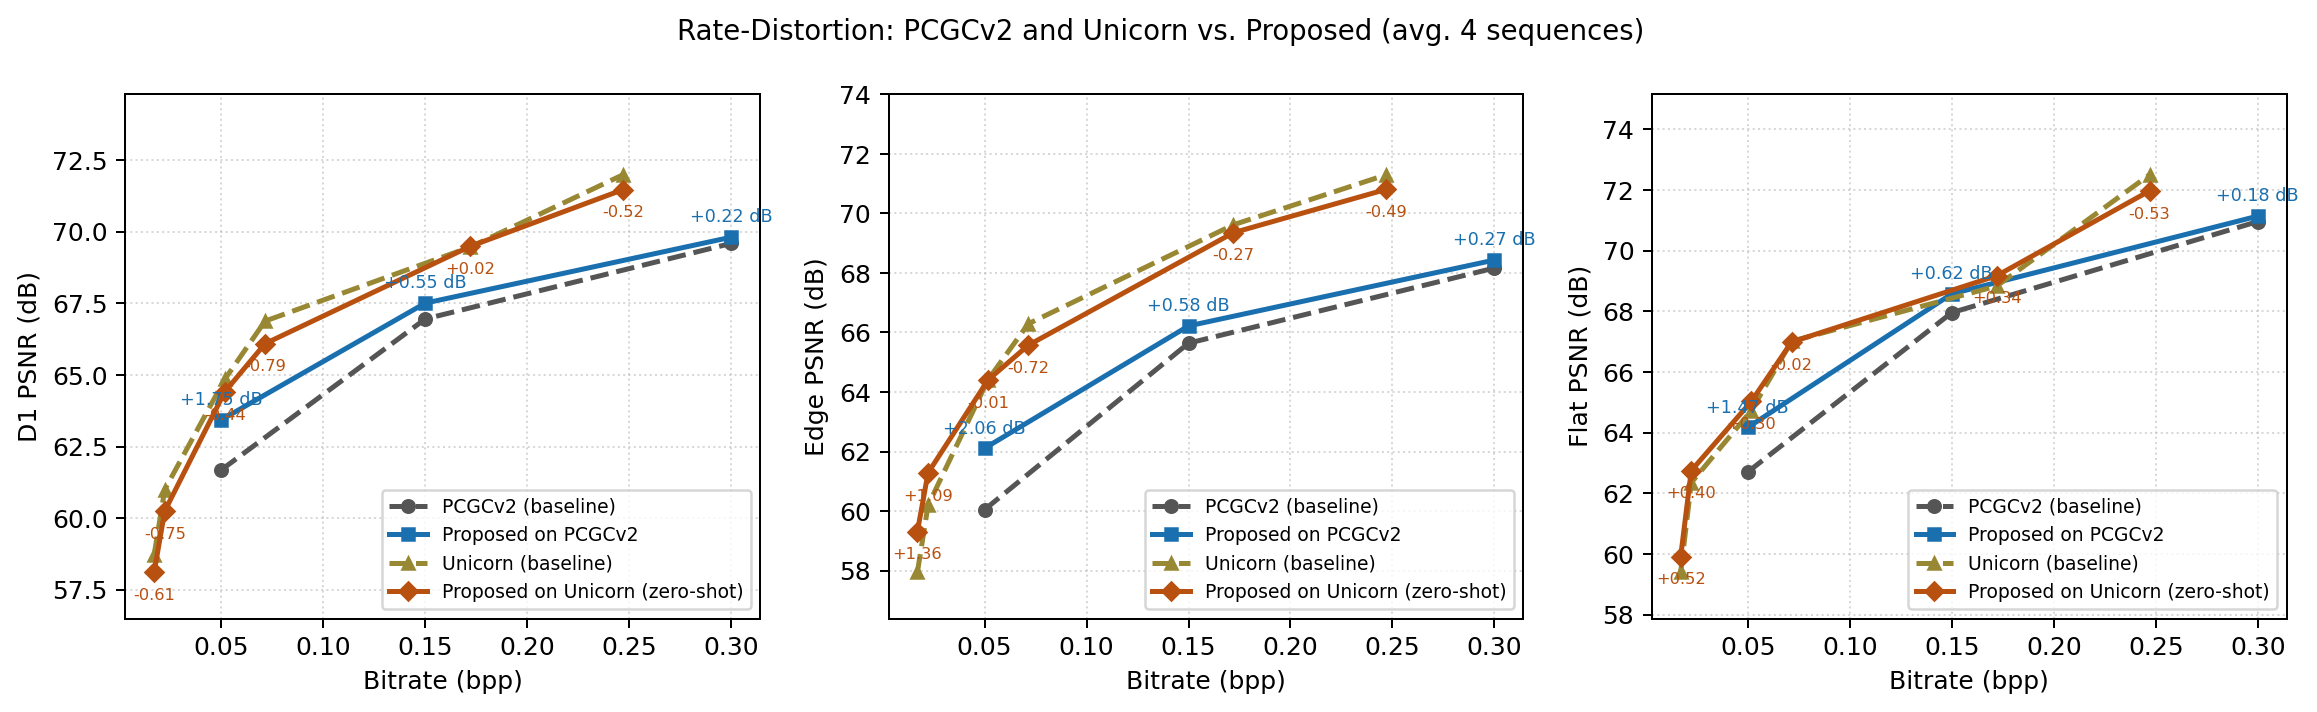
\includegraphics[width=\textwidth]{figures/rd_curve.png}
  \caption{Rate-distortion curves averaged over all four 8iVFB sequences (400 frames). Dashed lines are baselines; solid lines are the proposed method. PCGCv2 (blue) improves consistently across all three metrics. Unicorn zero-shot transfer (orange, 6 rate points R1--R6) is overlaid in Edge and Flat panels: the model improves below ${\approx}0.05$~bpp where oversmoothing is codec-agnostic, and degrades above it. Unicorn D1 (symmetric) does not improve even at low rates because the displacement corrections reduce forward error (hallucination) while improving reverse error (missing geometry); the edge and flat panels isolate this effect.}
  \label{fig:rd}
\end{figure*}

% --- Table I: Main results (directly below Fig 3) ---
\begin{table*}[!t]
  \centering
  \caption{Curvature-stratified PSNR gains over PCGCv2 baseline (dB), avg.\ 4 sequences (400 frames). BD-PSNR over r2/r4/r6.}
  \label{tab:main}
  \begin{tabular}{lccccccccc}
    \toprule
    & \multicolumn{2}{c}{r2 (0.05~bpp)} & \multicolumn{2}{c}{r4 (0.15~bpp)} & \multicolumn{2}{c}{r6 (0.30~bpp)} & \multicolumn{3}{c}{BD-PSNR (dB)} \\
    \cmidrule(lr){2-3} \cmidrule(lr){4-5} \cmidrule(lr){6-7} \cmidrule(lr){8-10}
    Method & Edge $\Delta$ & Flat $\Delta$ & Edge $\Delta$ & Flat $\Delta$ & Edge $\Delta$ & Flat $\Delta$ & D1 & Edge & Flat \\
    \midrule
    PCGCv2   & 0.00 & 0.00 & 0.00 & 0.00 & 0.00 & 0.00 & 0.00 & 0.00 & 0.00 \\
    Proposed & \textbf{+2.06} & \textbf{+1.47} & \textbf{+0.58} & \textbf{+0.62} & \textbf{+0.27} & \textbf{+0.18} & \textbf{+0.85} & \textbf{+0.97} & \textbf{+0.79} \\
    \bottomrule
  \end{tabular}
\end{table*}

% =============================================================================
\section{Experiments}
\label{sec:experiments}

\subsection{Setup}

We use the 8i Voxelized Full Bodies (8iVFB) dataset~\cite{8ivfb}, comprising
four sequences: \emph{longdress}, \emph{loot}, \emph{redandblack}, and
\emph{soldier}, each at $10$-bit voxel precision (grid size $1024^3$).
PCGCv2 is used as the baseline codec at three rate points (r2, r4, r6).
The model is trained on decoded frames from all four sequences using a
leave-one-out validation split (\emph{redandblack} held out), then evaluated
on all four. The full model has approximately 2.5M parameters and processes a
typical 8iVFB frame (${\approx}750$K points) in under 300~ms on a single GPU,
comparable in throughput to the decompression step itself. Despite the small training corpus (4 sequences, approximately 300
compressed frames across three rates), the model generalizes to held-out
sequences within 8iVFB and zero-shot to MVUB and Unicorn, suggesting the
corrections generalize beyond the training sequences. All quality measurements use peak value 1023 and $k{=}30$
for curvature stratification.

\subsection{Quantitative Results}

% --- Table 1: Main results ---
Table~\ref{tab:main} and Fig.~\ref{fig:rd} summarize results across all three
rate points (400 frames total). The method improves all four sequences at all
three rates. Gains are largest at r2 (+2.06~dB edge), where oversmoothing is
most severe. Edge improvement exceeds flat improvement (+1.47~dB) at r2,
confirming corrections concentrate on geometrically complex regions.
Gains decrease monotonically with rate: at r6 the codec already preserves fine
structure well, and the rate conditioning correctly suppresses large
displacements where aggressive corrections would introduce errors.
Fig.~\ref{fig:vis} shows a qualitative example at r2; surface protrusions lost
by compression are substantially recovered without changing overall shape.


% =============================================================================
% --- Tables II and III grouped together (page 5 top) ---
\begin{table*}[!t]
  \begin{minipage}[t]{0.42\linewidth}
    \centering
    \caption{Ablation on key design choices. Edge PSNR $\Delta$ at r2, avg.\ over 4 sequences (dB).}
    \label{tab:ablation}
    \begin{tabular}{lc}
      \toprule
      Configuration & Edge $\Delta$ (dB) \\
      \midrule
      Proposed (3-ch xyz, FiLM head, multi-rate) & \textbf{+2.06} \\
      w/ curvature input (4-ch features)          & +1.62 \\
      Single-rate model (r2 only)                 & +1.45 \\
      Full FiLM backbone (rate in all blocks)     & diverged \\
      \bottomrule
    \end{tabular}
  \end{minipage}
  \hfill
  \begin{minipage}[t]{0.55\linewidth}
    \centering
    \caption{Zero-shot generalization: Edge and Flat PSNR $\Delta$ (dB). Model trained on PCGCv2/8iVFB only; applied unchanged to Unicorn and MVUB.}
    \label{tab:generalization}
    \footnotesize
    \begin{tabular}{llcc}
      \toprule
      Setting & Sequence / Rate & Edge $\Delta$ & Flat $\Delta$ \\
      \midrule
      Cross-codec (Unicorn) & 8iVFB, R2 (0.17~bpp) & $-0.27$ & $+0.34$ \\
                            & 8iVFB, R3 (0.071~bpp) & $-0.72$ & $-0.02$ \\
                            & 8iVFB, R4 (0.052~bpp) & $-0.01$ & $+0.30$ \\
                            & 8iVFB, R5 (0.023~bpp) & $\mathbf{+1.09}$ & $\mathbf{+0.40}$ \\
      \midrule
      Cross-dataset (MVUB)  & david, r2   & $\mathbf{+0.92}$ & $\mathbf{+0.47}$ \\
                            & david, r4   & $-0.46$ & $-0.06$ \\
                            & david, r6   & $-0.09$ & $-0.09$ \\
                            & ricardo, r2 & $\mathbf{+1.03}$ & $\mathbf{+0.43}$ \\
                            & ricardo, r4 & $-0.50$ & $-0.14$ \\
                            & ricardo, r6 & $-0.12$ & $-0.12$ \\
      \bottomrule
    \end{tabular}
  \end{minipage}
\end{table*}

\subsection{Ablation Study}
\label{subsec:ablation}

Table~\ref{tab:ablation} isolates three design decisions. \textbf{Curvature
input}: replacing coordinate-only input with xyz+curvature reduces edge gain by
0.44~dB. We attribute this to the curvature estimator introducing noise at boundaries
(the same regions the model needs to correct) while the backbone already
encodes local geometry through its sparse convolution receptive field.
\textbf{Multi-rate training}: the single-rate model (r2 only) achieves
+1.45~dB, below the multi-rate variant; joint training across rates acts as a
regularizer. \textbf{Full FiLM backbone}: applying rate modulation to every
residual block caused gradient interference from mixed-rate batches in shared
weights; restricting modulation to the head resolves this.


\subsection{Cross-Codec and Cross-Dataset Generalization}
\label{subsec:generalization}

\textbf{Cross-codec (Unicorn)}: We apply the model trained on PCGCv2 output
to point clouds decoded by Unicorn~\cite{wang2025unicorn}, a structurally distinct
learned codec with a different entropy model and voxelization strategy. Rate
conditioning uses the actual decoded bitrate from Unicorn's output stream.
Results reveal a clear bitrate-dependent crossover (Table~\ref{tab:generalization}).
At 0.17--0.07~bpp (R2--R3), edge PSNR degrades ($-0.27$ to $-0.72$~dB): Unicorn's
distortion pattern at medium rates differs from the PCGCv2 training distribution,
causing overcorrection. At R4 (0.052~bpp), edge gain is essentially zero ($-0.01$~dB),
marking the crossover point. At R5 (0.023~bpp), both metrics improve substantially
($+1.09$ and $+0.40$~dB): at extreme compression, oversmoothing artifacts become
codec-agnostic and the learned corrections transfer. Flat PSNR remains positive even
at R2 ($+0.34$~dB), suggesting the backbone extracts transferable coarse geometry
features even when fine-structure corrections misfire.

\textbf{Cross-dataset (MVUB)}: We evaluate on two sequences from the Microsoft
Voxelized Upper Bodies dataset~\cite{loop2016mvub} (\emph{ricardo} and
\emph{david}), unseen during training. The model is applied without
modification. At r2, edge PSNR improves by $+0.92$~dB (david) and $+1.03$~dB
(ricardo); flat PSNR improves by $+0.47$ and $+0.43$~dB respectively. At r4
and r6, both metrics show degradation (${\approx}{-0.5}$~dB edge at r4),
which we attribute to two factors: the training distribution is heavily
weighted toward r2, and MVUB's higher point density (${\sim}1.5$M pts/frame
vs.\ ${\sim}800$K for 8iVFB) places the model out of its training range.
The strong r2 result confirms that low-rate oversmoothing corrections transfer
across human-body datasets with different capture rigs.
Results are summarized in Table~\ref{tab:generalization}.


% =============================================================================
\section{Conclusion and Future Work}
\label{sec:conclusion}

We presented a lightweight, rate-conditioned post-processing network for
learned point cloud compression. A FiLM-modulated prediction head lets a
single 2.5M-parameter model operate across multiple bitrates while the shared
backbone remains rate-invariant. Explicit curvature input is detrimental:
the backbone encodes local geometry from voxel coordinates, and curvature
adds noise at the boundaries the model is trying to correct. The
curvature-stratified PSNR metric exposes a quality gap at surface edges that
aggregate metrics miss; the proposed method closes that gap by +2.06~dB at
the lowest tested bitrate. Gains fall off at higher bitrates by design, and
zero-shot transfer to an unseen codec and dataset confirms the corrections
generalize across codec architectures.

The displacement formulation preserves point count by construction: the model
can only relocate existing decoded points and cannot recover geometry that the
codec dropped entirely or remove spurious extra points. At low bitrates,
PCGCv2 errors include both displacement errors (points slightly misplaced) and
occupancy errors (points wholly missing or hallucinated); the present method
addresses only the former.

One direction is to reformulate post-processing as \emph{occupancy prediction}:
given a dilated neighborhood of the decoded cloud as candidate voxels, predict
binary occupancy for each candidate. This eliminates displacement targets
entirely, directly addresses occupancy errors, and fits the integer voxel grid
on which learned codecs operate.

\section*{Acknowledgment}
This work was supported by the Research Committee of the Department of Electrical and Computer
Engineering, University of Patras.

\bibliographystyle{IEEEtran}
\bibliography{references}

\end{document}
